\documentclass[dvipdfmx]{beamer}
\usepackage{bxdpx-beamer}% dvipdfmxなので必要
\usepackage{pxjahyper}% 日本語で'しおり'したい
\renewcommand{\kanjifamilydefault}{\gtdefault}% 既定をゴシック体に


%% テーマ
\usetheme{metropolis}           % Use metropolis theme
%% 参照
\def\figref#1{図\ref{#1}}
\def\tblref#1{表\ref{#1}}
\def\eqref#1{式(\ref{#1})}

\newlength{\mytotalwidth}
\mytotalwidth=\dimexpr\linewidth-5mm
\newlength{\mycolumnwidth}
\mycolumnwidth=\dimexpr\mytotalwidth-5mm

\usepackage{graphicx}
\newcommand{\thickhrulefill}{\leavevmode\leaders\hrule depth-1.2pt height 3.2pt\hfill\kern0pt}
\newcommand{\indicatewidth}[1]{\thickhrulefill{#1}\thickhrulefill}
\usepackage{bm}
\usepackage{scalefnt}

\renewcommand{\figurename}{図}
\renewcommand{\tablename}{表}
\setbeamertemplate{caption}[numbered]

%% コンテンツ
\title{ 論文タイトル \cite{latex2e}}
\date{\today}
\author{\input{name.tex}}
\institute{}


\begin{document}
  \maketitle
  \section{数理計画問題 非線形}
  \begin{frame}{SOCP定式化}
    制約条件:再投影誤差=2次錘制約条件
    \begin{equation}
        \| 
        \frac{1}{\mathrm{\bm{p}}_3^{\mathrm{T}} \bm{Q}_i} \left(
        \begin{array}{c}
          \mathrm{\bm{p}}_1^{\mathrm{T}} \bm{Q}_i  \\
          \mathrm{\bm{p}}_2^{\mathrm{T}} \bm{Q}_i
        \end{array}
      \right)
     - \bm{q}_i^{\prime}\| \le \varepsilon_{\mathcal{I}}
     \label{eq:cons_tmp_img}
    \end{equation}

    3次元表面点の深度最大化問題→SOCP定式化可能 \\
    \begin{equation}
        \begin{aligned}
            & \underset{\bm{Q}} {\text{max}} && {\bm{p}}_3^{\mathrm{T}} \sum_{i=1}^{n_c} \bm{Q}\\
        &\text{subject to} &&
            \tiny
            \| 
            \left[
            \begin{array}{c}
              \mathrm{\bm{p}}_1^{\mathrm{T}}  \\
              \mathrm{\bm{p}}_2^{\mathrm{T}}
            \end{array}
            \right] \bm{Q}_i
          - \bm{q}_i^{\prime}\mathrm{\bm{p}}_3^{\mathrm{T}} \bm{Q}_i \| \le \varepsilon_{\mathcal{I}} \mathrm{\bm{p}}_3^{\mathrm{T}} \bm{Q}_i \normalsize &&& \forall i \in \{1, ..., n_c\}\\
        &                  && \| \bm{Q}_i -\bm{Q}_j\| \le d_{ij}  &&& \forall(i, j) \in \varepsilon \\
        &                  && \mathrm{\bm{p}}_3^{\mathrm{T}} \ge 0  &&&  \forall i \in \{1, ..., n_c\}
        \end{aligned}
        \label{eq:socp}
    \end{equation}
  \end{frame}
  \begin{frame}{frame環境で1枚のスライドができます.}
      とりあえず\\frame\{\}でスライドを作りましょう.
      セクションを宣言すると,大きいタイトルページが挿入されます.
      スライドのスタイルを変更すると良いと思います.
      プリアンブルにテーマと書いてあるところがあります.そこを参考に,beamerがサポートしているテーマを選べばOKです.
  \end{frame}
  \begin{frame}{図の挿入}
      図の挿入は普通のドキュメント通りには行かないみたいです.
      下の例を参考にコピペしてください.
     \begin{block}{}
         \centering
        \begin{columns}[onlytextwidth]
            \begin{column}[T]{0.49\textwidth} % 左:60%
                \centering
                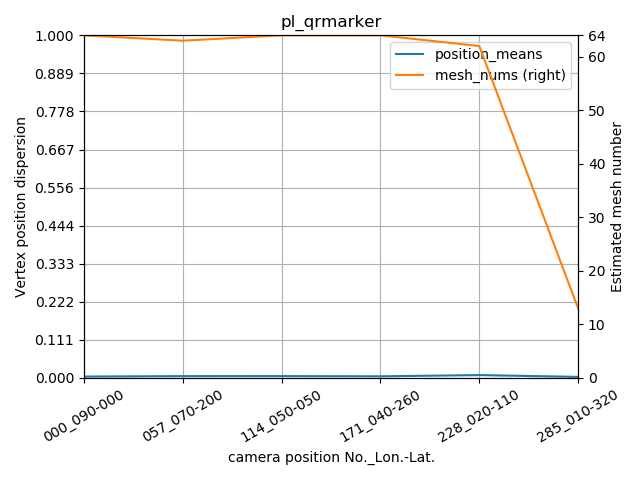
\includegraphics[width=1.0\linewidth]{img/fig.png}
                図a) 画像のれい
            \end{column}
            \begin{column}[T]{0.49\textwidth} % 右:40%
                \centering
                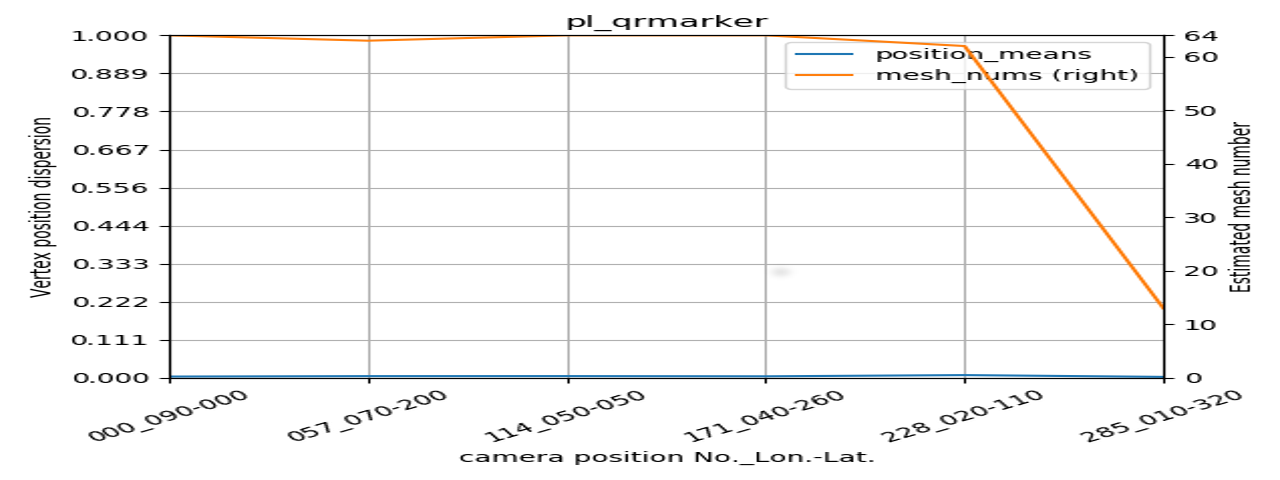
\includegraphics[width=1.0\linewidth]{img/fig-buchi.png}
                図b) 画像のれいその2
            \end{column}
        \end{columns}
        図1 キャプションを入れる
     \end{block}
  \end{frame}
  \begin{frame}{参考文献}
    \bibliographystyle{sieicej}
    \bibliography{library}%bibTexのファイル名
\end{frame}
\end{document}
